\documentclass[a4paper]{article}

%% Language and font encodings
\usepackage[english]{babel}
\usepackage[utf8x]{inputenc}
\usepackage[T1]{fontenc}

%% Sets page size and margins
\usepackage[a4paper,top=3cm,bottom=2cm,left=3cm,right=3cm,marginparwidth=1.75cm]{geometry}

% packages
\usepackage{amsmath, amsfonts}
\usepackage{graphicx, multicol}
\usepackage{textgreek,mathrsfs,bbm,relsize,multirow,float}
\usepackage{amssymb,amsthm,mathtools,scrextend,stackengine}
\usepackage[table,xcdraw]{xcolor} % clashes with tikz package
\usepackage[colorinlistoftodos]{todonotes}
\usepackage{wrapfig}
\newenvironment{frcseries}{\fontfamily{frc}\selectfont}{}
%% commands
\newcommand{\xbar}{\mbox{\larger$\bar{x}$}}
\renewcommand{\baselinestretch}{1.5} %%1.5 spacing
\newcommand{\textfrc}[1]{{\frcseries#1}}
% commands

\newenvironment{sbmatrix}[1]
 {\def\mysubscript{#1}\mathop\bgroup\begin{bmatrix}}
 {\end{bmatrix}\egroup_{\textstyle\mathstrut\mysubscript}}
 
\pgfdeclarelayer{background}
\pgfsetlayers{background,main}

\title{Stats Learning Lecture Week 5}

\begin{document}

\section{Notes}

\subsection{Trees}

In many cases, you might want to produce a model that can be easily visualized for clients and CEOs. One of the best models in machine learning for this is the trees algorithm (also known as CART, classification and regression trees). While you've already covered trees in another class, here we'll go into more detail on furthering the usage of trees.

Decision trees partition the input space into $q$ disjoint regions such that:
\begin{align}
\mathcal{X}&=R_i\cup R_2\cup\dots\cup R_q\\
&=\bigcup_{l=1}^{q}R_l
\end{align}

The prediction in each region in $R_l$ consists of a single constant, $f(x)$, which makes trees a piecewise constant function estimator.

This partitioning is created using the response variable and a criterion. At each split, variables are scanned and one is chosen to create a rule. A threshold is created with this variable and the splitting continues until reaching a stopping condition which determines a node to be a leaf. At each node, the label is determined by majority rule.

For binary classification, the most common criterion are:
\begin{align*}
\text{Misclassification}: & 1-\text{max}(p,1-p)\\
\text{Gini}: & 2p(1-p)\\
\text{Entropy/Likelihood}: &-p\text{log}(p)-(1-p)\text{log}(1-p)
\end{align*}

When running trees on the Pima Indian training set, we can produce the following trees diagram to show how the algorithm chunks up the data to determine predictions.

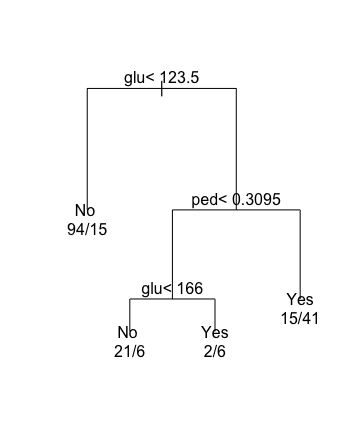
\includegraphics[scale=.6]{tree_diag.png}
** Short video explaining how each branch is a "linear divider" that splits the data to create the branches

A natural extension of trees is to create an ensemble of a bunch of trees to get better predictive power; this is called random forest.

\subsection{Random Forest}

In random forests, numerous trees are created and then aggregates across all the trees created to determine the classification of each observation. One of the defining features of random forest is that each subsequent tree in the ensemble should explain different aspects of the data, and that thus each tree should be orthogonal to each other. Random forest is extremely useful when there is a large number of attributes as well as for when forward/backward selection is inappropriate (due to correlation) to use to lessen the number of attributes. It is also 'embarrassingly parallel'. **** AIO on this phrase for a pop up explaining: "This means it lends itself very well to parallel computing thus greatly reducing computing time. This is accomplished by each tree in the ensemble being able to be computed at the same time since one tree does not affect how another is computed."

$$\hat{f}_{RF}^{(B)}(x^{\text{new}})\stackrel{\text{argmax}}{y\in Y}\Big\{\frac{1}{B}\{I(\hat{f}^{(b)}(x^{\text{new}})=y)\}\Big\}$$

For random forest, the general algorithm consists of creating each tree and storing them for aggregation when predicting:

for ($b=1$ to $B$)
\begin{itemize}
\item Draw a bootstrap sample from the data
\item Build the $b^{th}$ tree, $\hat{f}^{(b)}(\cdot)$
\begin{itemize}
\item at each node, only $q$ variables are considered (where there are a total of $p$ variables and $q\lll p$ and $q$ was selected a priori)
\item Select the best split $(x_{jk},\tau_k), k=1,\dots,q$ out of the q selected variables
\item Do not prune the tree
\item Store  $\hat{f}^{(b)}(\cdot)$
\end{itemize}
\item Aggregate predictions of the ensemble to make the final prediction of each observation in the test set
\end{itemize}

\subsubsection{Balanced Random Forest}

To accomplish balanced random forest, the class priors of the training set are set to be equal by forcing the number of observations in each class of the response to be equal. This is done either by reusing data points to artificially inflate the number of observations in a class, or by getting rid of observations to bring the number of observations down. Balanced random forest runs similarly to random forest but with one twist at the beginning of each iteration:

for ($b=1$ to $B$)
\begin{itemize}
\item Draw a bootstrap sample from the minority class with replacement and randomly draw the same amount from the majority class
\item Build the $b^{th}$ tree, $\hat{f}^{(b)}(\cdot)$
\begin{itemize}
\item at each node, only $q$ variables are considered (where there are a total of $p$ variables and $q\lll p$ and $q$ was selected a priori)
\item Select the best split $(x_{jk},\tau_k), k=1,\dots,q$ out of the q selected variables
\item Do not prune the tree
\item Store  $\hat{f}^{(b)}(\cdot)$
\end{itemize}
\item Aggregate predictions of the ensemble to make the final prediction of each observation in the test set
\end{itemize}

%\parencite{Chen2001} 

If your data shows an imbalance in the number of observations representing each class of the response, then you'll need to find a way to account for this in the algorithm itself. For random forest, that means either changing the weights of the classes observations to force the minor class observations to be equally important to the creation of the model as the major class observations (weighted random forest) or coercing the algorithm to use the same number of minor and major class observations (balanced random forest).

\subsubsection{Weighted Random Forest}


In weighted random forest, the goal is to place weights on the class priors of the response in the training set such that these class weights penalize misclassifying the minority class more than the majority class. This is accomplished by placing class weights in two places in the random forest algorithm: at each terminal node and at the final class prediction. Thus at each terminal node, predictions are made by weighted majority vote. The final class prediction is then made by aggregating these weighted votes in each individual tree. The individual trees are weighted by the average weight of all their terminal nodes.%\parencite{Chen2001}. 


\subsubsection{Oblique Random Forest}
Contrary to how random forest is done normally, oblique random forests takes on a different approach when creating the trees. Instead of having each tree explain different aspects about the data, they should randomly create hyperplanes chunking up the data. You can think of it similar to if you just kept placing more dividers on the data like in the original trees algorithm. Thus, the main difference here is that oblique random forest using multivariate models for the splits at each node instead of univariate models for the splits. In plain terms, this means that where random forest would normally only consider using a subset of the variables to create splits, oblique random forest uses all of the variables to determine the optimal split at each node. This means that for data with a very large number of attributes, many of which may be equally important, oblique random forest should perform better than regular random forest.


* Data sets in R/Python as examples

\subsection{Week 5 - Homeworks}
run through rf/trees with a few data sets
explain outcome differences
compare weighted to balanced and discuss which they prefer
compare outcomes via different metrics

\subsection{Week 5 - AIOS}
growing tree gif
video on optimizing trees and then another for RF (number of  nodes, number of features to try at each node)

** oblique, weighted, balanced rf papers, also the leo brieman trees paper for students to read to get more in depth knowledge on algorithms

\end{document}

